\documentclass{article}

\usepackage{amsmath}
\usepackage{graphicx}
\usepackage{tikz}
\usepackage{pgfplots}
\usepackage{xcolor}
 
\begin{document}

\title{AI Coffe Club (09/01/2020)\\ Activation Functions}
\date{}

\maketitle

\begin{center}
Last modification: \today\\
\end{center}

Activation functions are used to modify or control the output of layers of a neural network. More precisely, they are applied to each neuron and they determine whether they should be activated or not and, in more complex cases, the magnitude of such activation.

Although activation functions were traditionally used as a mathematical gate, a simple step function, to turn the neuron on and off depending on a threshold to produce binary classifications, nowadays they are used for more complex purposes.

Modern neural networks use non-linear activation functions to create complex mappings between the inputs and the output and generate more complex decision boundaries to tackle difficult classification problems.

Many activation functions have been proposed to date, most of them trying to strike a balance between making the training easier, increasing representation capacity, avoiding common training stalemates, and computational efficiency. Table \ref{table:activations} shows a summarized overview.

\textbf{Remark: we need activation functions to be differentiable so as to perform backpropagation optimization.}

\begin{table}[!htb]
  \centering
  \resizebox{\linewidth}{!}{
  \begin{tabular}{|c|c|c|c|}
    \hline
    Name & Function & Derivative & Range\\
    \hline
    Sigmoid & $\sigma(x) = \frac{1}{1 + e^{-x}}$ & $\sigma'(x) = \sigma(x)(1 - \sigma(x))$ & $(0,1)$\\
    \hline
    Hyperbolic Tangent & $\sigma(x) = \frac{e^{2x} -1}{e^{2x} + 1}$ & $\sigma'(x) = 1 - \sigma(x)^2$ & $(-1,1)$\\
    \hline
    ReLU & $\sigma(x) =
    \begin{cases}
      0 & x \leq 0\\
      x & x > 0
    \end{cases}$ & $\sigma(x) =
    \begin{cases}
      0 & x \leq 0\\
      x & x > 0
    \end{cases}$ & $[0, \infty)$\\
    \hline
    Leaky ReLU & $\sigma(x) =
    \begin{cases}
      0.01x & x \leq 0\\
      x & x > 0
    \end{cases}$ & $\sigma(x) =
    \begin{cases}
      0.01 & x \leq 0\\
      x & x > 0
    \end{cases}$ & $(-\infty, \infty)$\\
    \hline
    Parametric ReLU & $\sigma(x) =
    \begin{cases}
      \alpha x & x \leq 0\\
      x & x > 0
    \end{cases}$ & $\sigma(x) =
    \begin{cases}
      \alpha & x \leq 0\\
      x & x > 0
    \end{cases}$ & $(-\infty, \infty)$\\
    \hline
    ELU & $\sigma(x) =
    \begin{cases}
      \alpha(e^x -1) & x \leq 0\\
      x & x > 0
    \end{cases}$ & $\sigma(x) =
    \begin{cases}
      \alpha + \sigma(x) & x \leq 0\\
      x & x > 0
    \end{cases}$ & $(-\alpha, \infty)$\\
    \hline
    Softplus & $\sigma(x) = \ln(1 + e^x)$ & $\sigma'(x) = \frac{1}{1 + e^{-x}}$ & $(0, \infty)$\\
    \hline
    Swish & $\sigma(x) = \frac{x}{1 + e^{-\beta x}}$ & $\sigma'(x) = \beta\sigma(x) + \frac{1}{1 + e^{-\beta x}}(1 - \beta\sigma(x))$ & \\
    \hline
  \end{tabular}}
  \caption{Common activation functions.}
  \label{table:activations}
\end{table}

\clearpage

\section{Sigmoid}

\begin{figure}[!htb]
  \centering
  \begin{tikzpicture}
    \begin{axis}[
      width= \linewidth,
      axis lines= middle,
      legend pos= south east,
      xmax=4,
      xmin=-4,
      ymin=-4,
      ymax=4,
      samples=100]
      \addplot[blue, ultra thick]{(1 / (1 + e^(-x)))};
      \addplot[red, ultra thick]{((1 / (1 + e^(-x))) * (1.0 - (1 / (1 + e^(-x)))))};
      \legend{$\sigma(x)$, $\sigma'(x)$}
    \end{axis}
  \end{tikzpicture}
\end{figure}

\begin{equation}
\sigma(x) = \frac{1}{1 + e^{-x}}
\end{equation}

\begin{equation}
\sigma'(x) = \sigma(x)(1 - \sigma(x))
\end{equation}

\begin{itemize}
  \item Smooth gradient.
  \item Output values are bounded normalizing the output.
  \item Clear activations which easily saturate to the range extremes.
  \item \textcolor{red}{Vanishing gradients.} 
  \item \textcolor{red}{Not zero centered outputs.}
  \item \textcolor{red}{Computationally expensive.}
\end{itemize}

\clearpage

\section{Hyperbolic Tangent}

\begin{figure}[!htb]
  \centering
  \begin{tikzpicture}
    \begin{axis}[
      width= \linewidth,
      axis lines= middle,
      legend pos= south east,
      xmax=4,
      xmin=-4,
      ymin=-4,
      ymax=4,
      samples=100]
      \addplot[blue, ultra thick]{(tanh(x))};
      \addplot[red, ultra thick]{( 1 - tanh(x)^2)};
      \legend{$\sigma(x)$, $\sigma'(x)$}
    \end{axis}
  \end{tikzpicture}
\end{figure}

\begin{equation}
\sigma(x) = tanh(x) = \frac{e^x - e^{-x}}{e^x + e^{-x}} = \frac{e^{2x} -1}{e^{2x} + 1}
\end{equation}

\begin{equation}
\sigma'(x) = 1 - \sigma(x)^2
\end{equation}

\begin{itemize}
  \item Smooth gradient.
  \item Output values are bounded normalizing the output.
  \item Clear activations which easily saturate to the range extremes.
  \item Zero-centered outputs.
  \item \textcolor{red}{Vanishing gradients.} 
  \item \textcolor{red}{Computationally expensive.}
\end{itemize}

\clearpage

\section{Rectified Linear Unit}

\begin{figure}[!htb]
  \centering
  \begin{tikzpicture}
    \begin{axis}[
      width= \linewidth,
      axis lines= middle,
      legend pos= south east,
      xmax=4,
      xmin=-4,
      ymin=-4,
      ymax=4,
      samples=512]
      \addplot[blue, ultra thick]{
        ifthenelse(
          x < 0,
          0,
          x
        )
      };
      \addplot[red, ultra thick]{
        ifthenelse(
          x < 0,
          0,
          1
        )
      };
      \legend{$\sigma(x)$, $\sigma'(x)$}
    \end{axis}
  \end{tikzpicture}
\end{figure}

\begin{equation}
\sigma(x) =
  \begin{cases}
    0 & x \leq 0\\
    x & x > 0
  \end{cases}
\end{equation}

\begin{equation}
\sigma'(x) =
  \begin{cases}
    0 & x \leq 0\\
    1 & x > 0
  \end{cases}
\end{equation}

\begin{itemize}
  \item Computationally efficient.
  \item Not affected by the vanishing gradient and converges faster.
  \item Sparse activations.
  \item \textcolor{red}{Unbounded output values.}
  \item \textcolor{red}{Dying ReLU}  since it is zero for all negative values and the slope in the negative range is zero it can "die". A large gradient flowing through a ReLU can cause the weights to update in such a way that the neuron will never activate on any datapoint again. The gradient flowing through this unit will be forever zero.
\end{itemize}

\clearpage

\section{Leaky Rectified Linear Unit}

\begin{figure}[!htb]
  \centering
  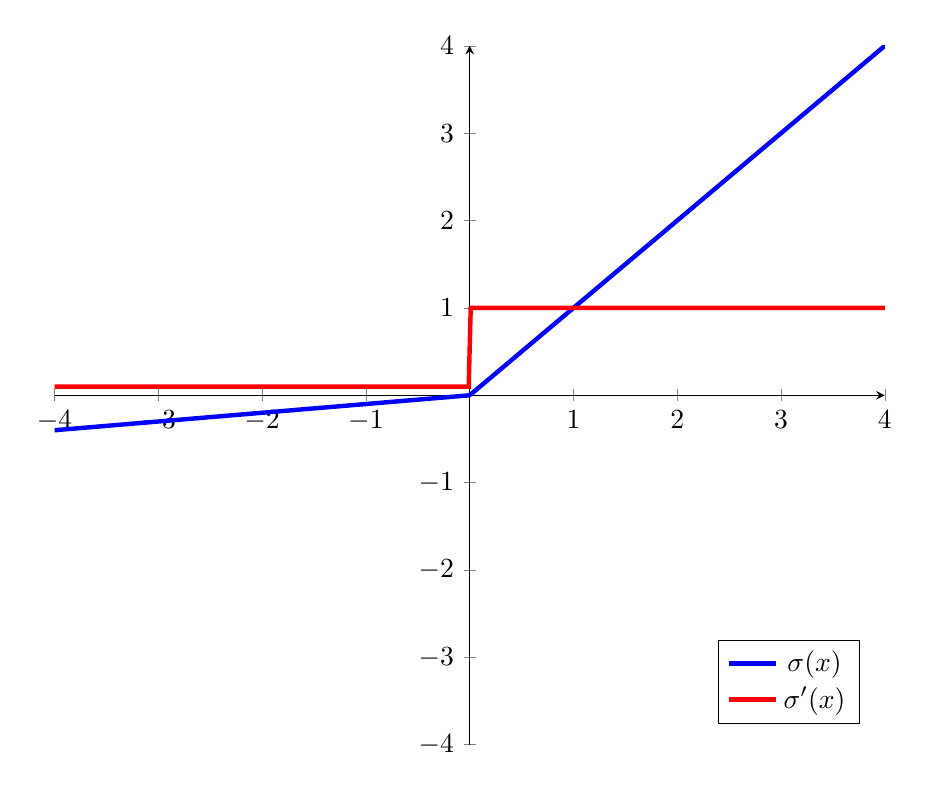
\begin{tikzpicture}
    \begin{axis}[
      width= \linewidth,
      axis lines= middle,
      legend pos= south east,
      xmax=4,
      xmin=-4,
      ymin=-4,
      ymax=4,
      samples=512]
      \addplot[blue, ultra thick]{
        ifthenelse(
          x < 0,
          0.1 * x,
          x
        )
      };
      \addplot[red, ultra thick]{
        ifthenelse(
          x < 0,
          0.1,
          1
        )
      };
      \legend{$\sigma(x)$, $\sigma'(x)$}
    \end{axis}
  \end{tikzpicture}
\end{figure}

\begin{equation}
  \sigma(x) =
    \begin{cases}
      0.1x & x \leq 0\\
      x & x > 0
    \end{cases}
\end{equation}
  
\begin{equation}
  \sigma'(x) =
    \begin{cases}
      0.1 & x \leq 0\\
      1 & x > 0
    \end{cases}
\end{equation}

\begin{itemize}
  \item Computationally efficient.
  \item Not affected by the vanishing gradient and converges faster.
  \item Prevents the dying ReLU problem!
  \item Sparse activations.
  \item \textcolor{red}{Not zero-centered.}
  \item \textcolor{red}{Unbounded output values.}
  \item \textcolor{red}{Inconsistent results due to inconsistent predictions for negative values.}
\end{itemize}

\clearpage

\section{Parametric Rectified Linear Unit}

\begin{figure}[!htb]
  \centering
  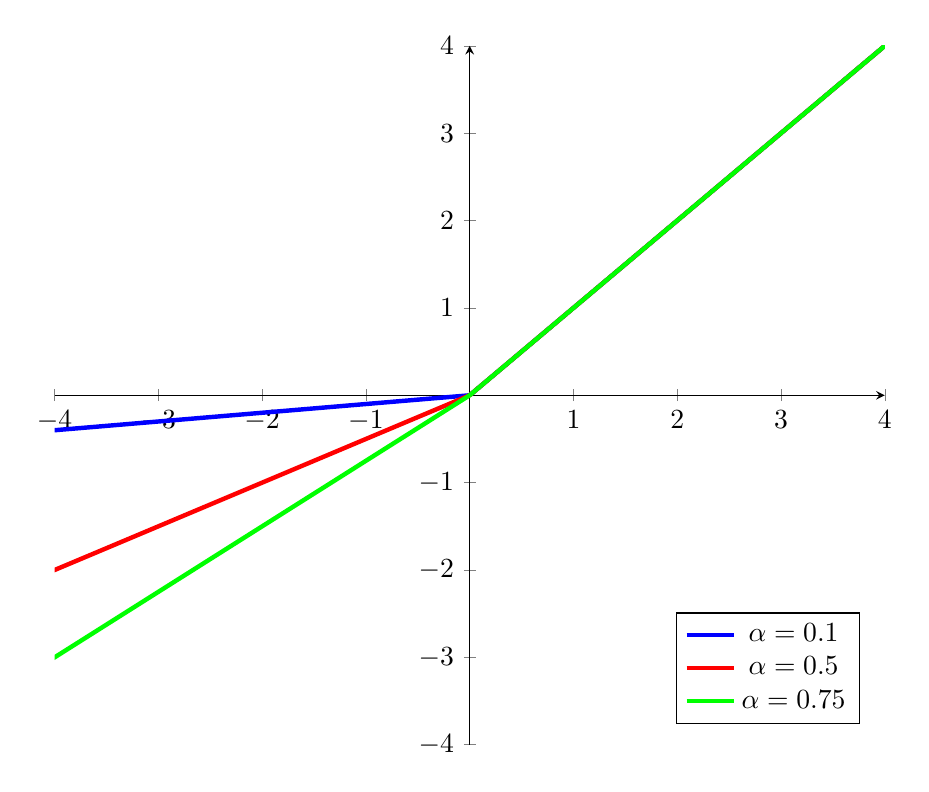
\begin{tikzpicture}
    \begin{axis}[
      width= \linewidth,
      axis lines= middle,
      legend pos= south east,
      xmax=4,
      xmin=-4,
      ymin=-4,
      ymax=4,
      samples=512]
      \addplot[blue, ultra thick]{
        ifthenelse(
          x < 0,
          0.1 * x,
          x
        )
      };
      \addplot[red, ultra thick]{
        ifthenelse(
          x < 0,
          0.5 * x,
          x
        )
      };
      \addplot[green, ultra thick]{
        ifthenelse(
          x < 0,
          0.75 * x,
          x
        )
      };
      \legend{$\alpha=0.1$, $\alpha=0.5$, $\alpha=0.75$}
    \end{axis}
  \end{tikzpicture}
\end{figure}

\begin{equation}
  \sigma(x) =
    \begin{cases}
      \alpha x & x \leq 0\\
      x & x > 0
    \end{cases}
\end{equation}

\begin{equation}
  \sigma'(x) =
    \begin{cases}
      \alpha & x \leq 0\\
      1 & x > 0
    \end{cases}
\end{equation}

\begin{itemize}
  \item Computationally efficient.
  \item Not affected by the vanishing gradient and converges faster.
  \item Prevents the dying ReLU problem!
  \item Sparse activations.
  \item Negative slope is learned and backpropagation is performed with the most appropriate value.
  \item \textcolor{red}{Not zero-centered.}
  \item \textcolor{red}{Unbounded output values.}
\end{itemize}

\clearpage

\section{Exponential Linear Unit}

\begin{figure}[!htb]
  \centering
  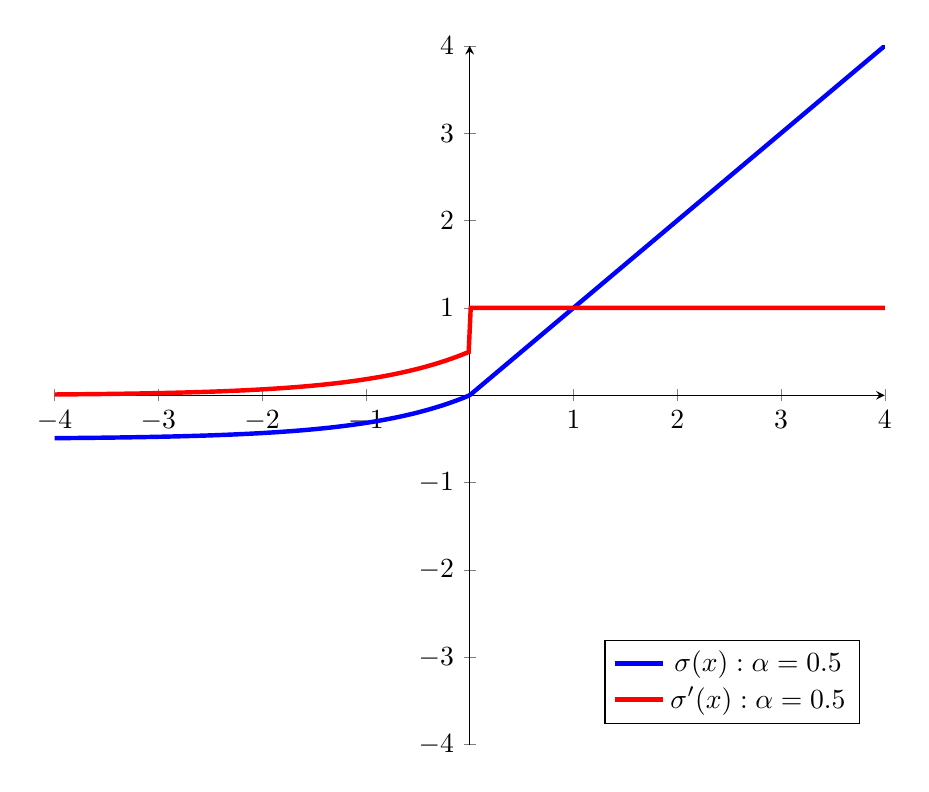
\begin{tikzpicture}
    \begin{axis}[
      width= \linewidth,
      axis lines= middle,
      legend pos= south east,
      xmax=4,
      xmin=-4,
      ymin=-4,
      ymax=4,
      samples=512]
      \addplot[blue, ultra thick]{
        ifthenelse(
          x < 0,
          0.5 * (e^x -1),
          x
        )
      };
      \addplot[red, ultra thick]{
        ifthenelse(
          x < 0,
          0.5 + 0.5 * (e^x -1),
          1
        )
      };
      \legend{$\sigma(x): \alpha = 0.5$, $\sigma'(x): \alpha = 0.5$}
    \end{axis}
  \end{tikzpicture}
\end{figure}

\begin{equation}
  \sigma(x) =
    \begin{cases}
      \alpha(e^x - 1) & x \leq 0\\
      x & x > 0
    \end{cases}
\end{equation}

\begin{equation}
  \sigma'(x) =
    \begin{cases}
      \alpha + \sigma(x) & x \leq 0\\
      1 & x > 0
    \end{cases}
\end{equation}

\begin{itemize}
  \item Computationally efficient.
  \item Not affected by the vanishing gradient and converges faster.
  \item Prevents the dying ReLU problem!
  \item Sparse activations.
  \item Negative slope is learned and backpropagation is performed with the most appropriate value.
  \item Smooth negative slope.
  \item \textcolor{red}{Not zero-centered.}
  \item \textcolor{red}{Unbounded output values.}
\end{itemize}

\clearpage

\section{Softplus}

\begin{figure}[!htb]
  \centering
  \begin{tikzpicture}
    \begin{axis}[
      width=\linewidth,
      axis lines= middle,
      legend pos= south east,
      xmax=4,
      xmin=-4,
      ymin=-4,
      ymax=4,
      samples=100]
      \addplot[blue, ultra thick]{(ln(1 + e^x))};
      \addplot[red, ultra thick]{(1.0 / (1 + e^(-x)))};
      \legend{$\sigma(x)$, $\sigma'(x)$}
    \end{axis}
  \end{tikzpicture}
\end{figure}

\begin{equation}
  \sigma(x) = \ln(1 + e^x)
\end{equation}

\begin{equation}
  \sigma'(x) = \frac{1}{1 + e^{-x}}
\end{equation}

\begin{itemize}
  \item All the advantages of sigmoid/tanh.
  \item No vanishing gradients.
  \item \textcolor{red}{Computationally inefficient}.
\end{itemize}

\clearpage

\section{Swish}

\begin{figure}[!htb]
  \centering
  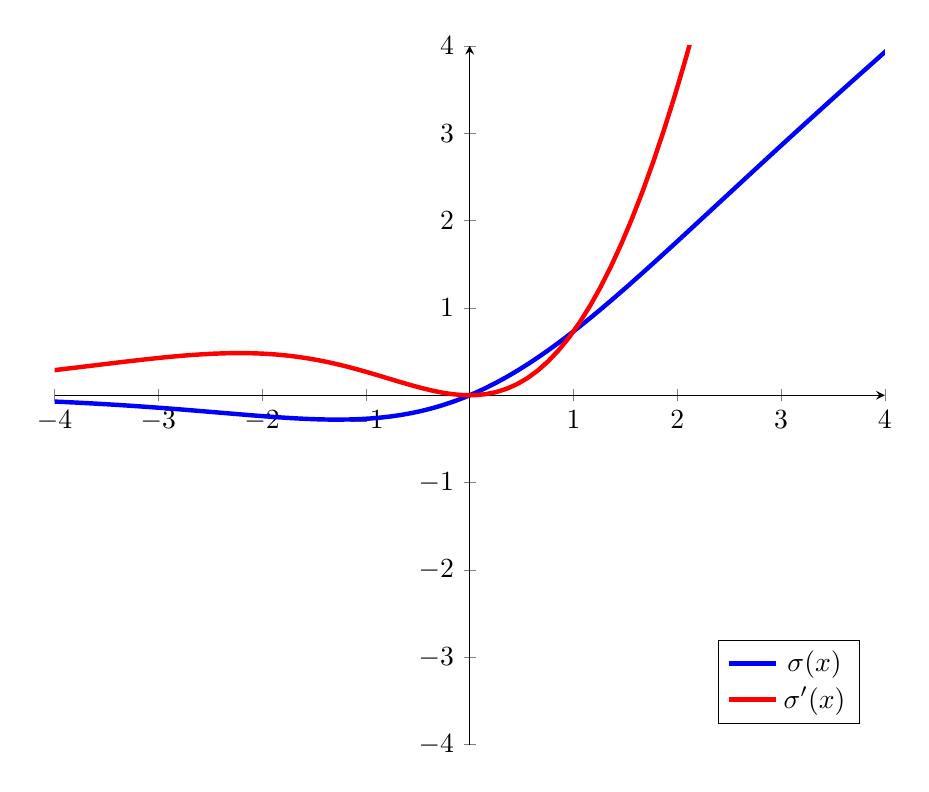
\begin{tikzpicture}
    \begin{axis}[
      width=\linewidth,
      axis lines= middle,
      legend pos= south east,
      xmax=4,
      xmin=-4,
      ymin=-4,
      ymax=4,
      samples=100]
      \addplot[blue, ultra thick]{(x / (1 + e^(-x)))};
      \addplot[red, ultra thick]{(x * (x / (1 + e^(-x))))};
      \legend{$\sigma(x)$, $\sigma'(x)$}
    \end{axis}
  \end{tikzpicture}
\end{figure}

\begin{equation}
\sigma(x) = \frac{x}{1 + e^{-x}}
\end{equation}

\begin{equation}
\sigma'(x) = x\sigma(x)
\end{equation}

\begin{itemize}
  \item All the advantages of sigmoid/tanh.
  \item Similar behaviour to ReLU but smooth.
  \item \textcolor{red}{Computationally inefficient}.
\end{itemize}

\end{document}